\documentclass{article}

\usepackage{times}
\usepackage{geometry}
\geometry{a4paper,left=0.6cm,right=0.7cm,top=2cm,bottom=1cm,columnsep=0.8cm}
\usepackage{fontawesome}
\usepackage[hidelinks]{hyperref}
\usepackage{multicol}
\usepackage{tikz}
\usepackage{hyphsubst}
\usepackage{moresize}
\usepackage{hyphenat}
\usepackage{tabularx}
\usepackage{xcolor}
\usepackage{enumitem}

\newcolumntype{Y}{>{\RaggedRight\arraybackslash}X}

\setlist[itemize]{itemsep=1pt,leftmargin=*,topsep=-10pt}

\definecolor{maincolor}{HTML}{f0fafc}
\definecolor{seccolor}{HTML}{ffffff}
\definecolor{gray}{HTML}{8c94a9}
\definecolor{sidetext}{HTML}{59cee5}

\usepackage[contents={}]{background}
\AddEverypageHook{\begin{tikzpicture}[remember picture,overlay]%
  \node[inner sep=0pt,outer sep=0pt] at (current page.north west) [anchor=north west]{%
  \fcolorbox{maincolor}{maincolor}{%
\begin{minipage}[t][\paperheight][t]{0.3\paperwidth}
        \color{white}
        \hspace{0.08cm}
\end{minipage}}
\fcolorbox{seccolor}{seccolor}{
\begin{minipage}[t][\paperheight][t]{0.67\paperwidth}
        \color{black}
        \hspace{1cm}
\end{minipage}
}
  };%
\end{tikzpicture}
}

\setlist[itemize]{itemsep=-2pt,topsep=0pt,leftmargin=1.08cm}
\renewcommand{\labelitemi}{\textcolor{sidetext}{\footnotesize$\bullet$}}

\setlength{\parindent}{0pt}
\usepackage{paracol}

\begin{document}

\pagestyle{empty}

\columnratio{0.3}
\begin{paracol}{2}
\color{sidetext}
\begin{center}
            \begin{tikzpicture}
            \clip (0,0) circle (1.5cm) node[anchor=center] {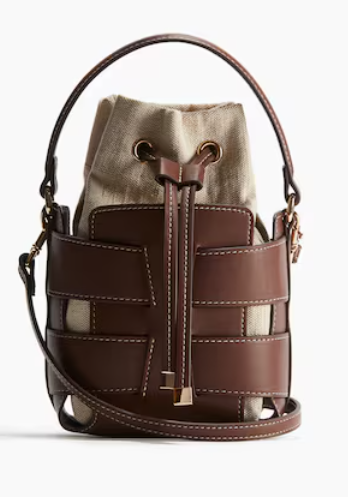
\includegraphics[width=3cm]{a87c3f3e57e74793b2fe3a77a91ccd31.png}}; 
            \end{tikzpicture}

            ~

         {\color{black}\LARGE \textbf{Pape FALL}}

         ~

         {\large{Data Scientist}}

        
        \end{center}

{\color{gray}\rule{\linewidth}{0.4pt}} \\

 \begin{tabular}{cl}
            \faPhone{}      & 
            \begin{tabular}{p{0.7\linewidth}}
            {\color{gray}Téléphone}\\
            {0753481453}
            \end{tabular}
            \\ \\
               \faLinkedin{}      & 
            \begin{tabular}{p{0.7\linewidth}}
            {\color{gray}LinkedIn}\\
            {\href{https://www.linkedin.com/in/pape}{https://www.linkedin.com/in/pape}}
            \end{tabular}
            \\ \\
               \faMapMarker{}      & 
            \begin{tabular}{p{0.7\linewidth}}
            {\color{gray}Adresse}\\
            {}
            \end{tabular}
            \\ \\
               \faGlobe{}      & 
            \begin{tabular}{p{0.7\linewidth}}
            {\color{gray}Site Web}\\
            {}
            \end{tabular}
            \\
        \end{tabular}
        \vspace{.2cm} \\
        {\color{gray}\rule{\linewidth}{0.4pt}} \\

        {\color{black}{Langues}}

        ~
        
        \begin{tabular}{cl}
            {\Large\faLanguage{}} & \begin{tabular}{l}
             Français \\
             {\color{gray}Courant}
            \end{tabular} \\
        \end{tabular}
        \vspace{10pt} \\
        {\color{gray}\rule{\linewidth}{0.4pt}} \\

        \vspace{.4cm}

        {\color{black}{Compétences clés}}

        ~
        
        \begin{tabular}{ll}
         \begin{minipage}{0.1\linewidth}
         
\includegraphics[width=\linewidth]{picon.png}
         \end{minipage} & Python, R, SQL \\[10pt]
         \begin{minipage}{0.1\linewidth}
         
\includegraphics[width=\linewidth]{picon.png}
         \end{minipage} & Machine Learning \\[10pt]
         \begin{minipage}{0.1\linewidth}
         
\includegraphics[width=\linewidth]{picon.png}
         \end{minipage} & Deep Learning \\[10pt]
         \begin{minipage}{0.1\linewidth}
         
\includegraphics[width=\linewidth]{picon.png}
         \end{minipage} & Data Visualisation (Matplotlib, Seaborn, Plotly) \\[10pt]
         \begin{minipage}{0.1\linewidth}
         
\includegraphics[width=\linewidth]{picon.png}
         \end{minipage} & AWS, Docker, Git \\[10pt]
        \end{tabular}
        
\switchcolumn
\color{black}

\textcolor{black}{\Large \textbf{Profil Professionnel}} \\

\textcolor{black}{Data Scientist with strong expertise in machine learning, statistical modelling and data storytelling, with experience delivering data-driven solutions in the telecommunications sector. Adept at translating complex datasets into actionable insights to drive strategic decision-making and business value.}\\[8pt]

\textcolor{black}{\Large \textbf{Expérience Professionnelle}} \\

\colorbox{maincolor}{%
  \begin{minipage}{\linewidth}
    \begin{tabular}{@{}lp{0.72\linewidth}r}
      \begin{minipage}{0.05\linewidth}
        
\includegraphics[width=\linewidth]{picon.png}
      \end{minipage} & 
      Prepaya &  
      {\footnotesize Jan 2022 -- Déc 2023 } \\[-10pt]
      & {\color{sidetext}{Data Scientist}} & \\
      & {\small Paris, France } & \\
    \end{tabular}
\begin{itemize}
    \item Développement de modèles prédictifs pour optimiser l’attrition client, entraînant une réduction du churn de 15 \%.
    \item Conception et déploiement de pipelines de machine learning évolutifs sous Python, scikit-learn et AWS.
    \item Collaboration avec des équipes pluridisciplinaires pour transformer les problématiques métiers en solutions analytiques.
    \item Automatisation des flux d’ingestion et de pré-traitement de données, réduisant de 40 \% le temps de génération des rapports.
\end{itemize}
  \end{minipage}%
}

\vspace{1cm}

\textcolor{black}{\Large \textbf{Formation}} \\


 \begin{tabular}{@{}cp{0.7\linewidth}}
      \begin{minipage}{0.05\linewidth}
        
\includegraphics[width=\linewidth]{picon.png}
      \end{minipage} & \vspace{-12pt}
      {\color{sidetext} Master 2 Data Science} \\[-6pt]
      & Sorbonne Université \\ 
      & Data Science \\ 
      & 2015 
    \end{tabular}

\vspace{0.5cm}

% Section Certifications supprimée

\end{paracol}

\end{document}